\documentclass[11pt]{article}

\usepackage[margin=1.05in]{geometry}
\usepackage{amsmath,amssymb,amsthm}
\usepackage{booktabs}
\usepackage{graphicx}
\usepackage{subcaption}
\usepackage{microtype}
\usepackage{natbib}
\usepackage[colorlinks=true,linkcolor=blue!55!black,citecolor=blue!55!black,
            urlcolor=blue!55!black]{hyperref}
\usepackage{cleveref}
\usepackage{xcolor}
\usepackage{algorithm}
\usepackage[noend]{algpseudocode}
\usepackage{enumitem}
\usepackage[section]{placeins}

\newtheorem{theorem}{Theorem}
\newtheorem{proposition}[theorem]{Proposition}
\newtheorem{lemma}[theorem]{Lemma}
\newtheorem{corollary}[theorem]{Corollary}
\theoremstyle{definition}
\newtheorem{definition}[theorem]{Definition}
\newtheorem{remark}[theorem]{Remark}

\newcommand{\R}{\mathbb{R}}
\newcommand{\E}{\mathbb{E}}
\newcommand{\Var}{\operatorname{Var}}
\newcommand{\Loss}{\mathcal{L}}
\newcommand{\Rec}{\mathcal{R}}
\newcommand{\D}{\mathcal{D}}
\newcommand{\Plane}{\mathcal{S}}
\newcommand{\bs}{\boldsymbol}
\newcommand{\lean}[1]{\texttt{#1}}

% Generated by paper/make_numbers.py -- do not edit.

\newcommand{\CNNanalysispts}{4{,}234}
\newcommand{\CNNanalysisradius}{35}
\newcommand{\CNNanalysisrange}{11.63}
\newcommand{\CNNbandwidth}{88.8}
\newcommand{\CNNbudgetdecades}{2.3}
\newcommand{\CNNbudgetgain}{\textcolor{red}{[pending]}}
\newcommand{\CNNbudgetmax}{3{,}339{,}659}
\newcommand{\CNNbudgetmin}{15{,}040}
\newcommand{\CNNdres}{37}
\newcommand{\CNNfullmax}{479.3}
\newcommand{\CNNkappaOne}{3.9}
\newcommand{\CNNkappaTwo}{20.8}
\newcommand{\CNNnoisenorm}{0.00654}
\newcommand{\CNNoverhead}{-3.3\%}
\newcommand{\CNNoverheadtotal}{124.2\%}
\newcommand{\CNNparams}{402{,}986}
\newcommand{\CNNradius}{40.44}
\newcommand{\CNNrangetrain}{479}
\newcommand{\CNNresidCentered}{5.85}
\newcommand{\CNNresidEndpoint}{7.04}
\newcommand{\CNNresidOrigin}{6.45}
\newcommand{\CNNrhoCentered}{0.8689}
\newcommand{\CNNrhoEndpoint}{0.8689}
\newcommand{\CNNrhoOrigin}{0.9753}
\newcommand{\CNNseeds}{3}
\newcommand{\CNNsharpfloor}{5.3}
\newcommand{\CNNsharpworst}{41}
\newcommand{\CNNsnaps}{302}
\newcommand{\CNNstencilk}{2.51}
\newcommand{\CNNtailshare}{39.9\%}
\newcommand{\CNNtauTwo}{548}
\newcommand{\CNNtauZero}{70.2}
\newcommand{\CNNtrainanchors}{83}
\newcommand{\CNNtraincertrel}{0.4\%}
\newcommand{\CNNtrainsec}{183}
\newcommand{\CNNtraintruerel}{2.2\%}
\newcommand{\CNNtrajgib}{0.68}
\newcommand{\CNNtrajinside}{100.0\%}
\newcommand{\CNNtrajmax}{4.22}
\newcommand{\CNNtrustfrac}{47.4\%}
\newcommand{\CNNtrustmin}{3.3\%}
\newcommand{\CNNtrusttol}{0.0483}
\newcommand{\CNNusec}{8.21}
\newcommand{\CNNvalanchors}{59}
\newcommand{\CNNvalcertrel}{3.5\%}
\newcommand{\CNNvaltruerel}{3.0\%}
\newcommand{\CNNvres}{75}
\newcommand{\Coverage}{99.6\%}
\newcommand{\ExpGGrid}{0.633}
\newcommand{\ExpGGridr}{-0.29}
\newcommand{\ExpGLsq}{0.274}
\newcommand{\ExpGOne}{0.171}
\newcommand{\ExpGRbf}{0.0937}
\newcommand{\ExpGTwo}{0.0527}
\newcommand{\ExpHGrid}{0.443}
\newcommand{\ExpHGridr}{-0.695}
\newcommand{\ExpHLsq}{0.189}
\newcommand{\ExpHOne}{0.126}
\newcommand{\ExpHRbf}{0.219}
\newcommand{\ExpHTwo}{0.131}
\newcommand{\ExpLGrid}{0.707}
\newcommand{\ExpLGridr}{0.169}
\newcommand{\ExpLLsq}{0.302}
\newcommand{\ExpLOne}{0.259}
\newcommand{\ExpLRbf}{0.152}
\newcommand{\ExpLTwo}{0.112}
\newcommand{\GPTanalysispts}{1{,}089}
\newcommand{\GPTanalysisradius}{68.1}
\newcommand{\GPTanalysisrange}{9.664}
\newcommand{\GPTbudgetdecades}{1.8}
\newcommand{\GPTbudgetgain}{\textcolor{red}{[pending]}}
\newcommand{\GPTbudgetmax}{919{,}300}
\newcommand{\GPTbudgetmin}{14{,}364}
\newcommand{\GPTdres}{13}
\newcommand{\GPTfullmax}{9.664}
\newcommand{\GPTkappaOne}{3.68}
\newcommand{\GPTkappaTwo}{28.1}
\newcommand{\GPTnoisenorm}{0.0266}
\newcommand{\GPToverhead}{14.2\%}
\newcommand{\GPToverheadtotal}{89.8\%}
\newcommand{\GPTparams}{5{,}018{,}112}
\newcommand{\GPTradius}{68.06}
\newcommand{\GPTrangetrain}{9.66}
\newcommand{\GPTresidCentered}{5.53}
\newcommand{\GPTresidEndpoint}{7.87}
\newcommand{\GPTresidOrigin}{6.66}
\newcommand{\GPTrhoCentered}{0.9438}
\newcommand{\GPTrhoEndpoint}{0.9438}
\newcommand{\GPTrhoOrigin}{0.9907}
\newcommand{\GPTseeds}{3}
\newcommand{\GPTsharpfloor}{62}
\newcommand{\GPTsharpworst}{113}
\newcommand{\GPTsnaps}{202}
\newcommand{\GPTstencilk}{2.51}
\newcommand{\GPTtauTwo}{0}
\newcommand{\GPTtauZero}{0.28}
\newcommand{\GPTtrainanchors}{114}
\newcommand{\GPTtraincertrel}{0.7\%}
\newcommand{\GPTtrainsec}{898}
\newcommand{\GPTtraintruerel}{0.7\%}
\newcommand{\GPTtrajgib}{5.66}
\newcommand{\GPTtrajinside}{100.0\%}
\newcommand{\GPTtrajmax}{8.91}
\newcommand{\GPTtrustfrac}{4.6\%}
\newcommand{\GPTtrustmin}{1.5\%}
\newcommand{\GPTtrusttol}{0.0632}
\newcommand{\GPTusec}{303}
\newcommand{\GPTvalanchors}{76}
\newcommand{\GPTvalcertrel}{0.9\%}
\newcommand{\GPTvaltruerel}{0.9\%}
\newcommand{\GPTvres}{33}
\newcommand{\GramSpeedup}{3.08}
\newcommand{\GramVsTriton}{14.7}
\newcommand{\PUspeedup}{225}
\newcommand{\PeakBW}{672.1}


\title{\bf Cheap \emph{and} Accurate Loss-Landscape Visualisation:\\
Budget-Optimal Probing with a Certified Error}

\author{}
\date{}

\begin{document}
\maketitle

\begin{abstract}
\noindent
Loss-landscape figures are read quantitatively --- for the width of a basin, the
direction of the gradient field, the sharpness of a minimum --- yet are produced without
any statement of their own accuracy. We pose the problem as budgeted stochastic function
estimation on a $2$-plane and derive what a compute budget $C$, in
example-forward-equivalents, can buy. Two facts drive the result. On a $2$-plane the
exact restricted gradient and the exact $2\times2$ restricted Hessian cost one backward
pass and two Hessian-vector products, independently of model size, so a single probe
yields a complete second-order Taylor model. And splitting $C$ between the number of
probes and the depth of each has a closed-form optimum: a partition-of-unity Taylor
reconstruction is best at $n^\star\!\propto\! C^{1/4}$ anchors, with error decaying as
$C^{-3/8}$ --- the nonparametric minimax rate for the smoothness assumed. The same
analysis shows that plotting a grid of noisy loss values, which is standard practice, is
an \emph{interpolating} estimator whose error cannot fall below the per-point
Monte-Carlo noise, and that curvature read off such a grid converges at $C^{-1/8}$
against $C^{-1/4}$ for direct Hessian probing. Every rendered surface ships with a
variance-corrected hold-out certificate, unbiased for its own mean squared error and
carrying a distribution-free confidence bound. On a \CNNparams-parameter CNN (CIFAR-10)
and a \GPTparams-parameter transformer (WikiText-2), scored against exact full-dataset
references, the measured exponents track the predicted ones and the $95\%$ bound holds
in \Coverage{} of runs. Six load-bearing lemmas are machine-checked in Lean~4.
\end{abstract}

\section{Introduction}
\label{sec:intro}

A loss-landscape figure is a claim about geometry. Readers use them to argue that one
minimum is flatter than another, that a barrier separates two solutions, that an
optimiser was pushed in a particular direction. Those are quantitative claims, and they
are made from pictures that carry no error bar.

The pictures are also expensive. Producing an $n\times n$ grid of loss values costs
$n^2$ passes over data; at $n=100$ and a dataset of $10^4$ examples that is $10^8$
example-forward-passes for a single frame. The response in practice is to shrink the
per-point sample --- a mini-batch instead of the dataset --- and this is where the
trouble starts, because it trades a cost that is visible for an error that is not.

\paragraph{The question.} We think the right question is not \emph{how do I interpolate
a sparse grid cheaply}, but:

\begin{quote}
Given a compute budget $C$, what is the smallest achievable error of a rendered loss
surface, and which sampling and reconstruction strategy achieves it?
\end{quote}

Posed this way the problem has a definite answer, and the answer contradicts common
practice in three specific ways.

\paragraph{Contributions.}
\begin{enumerate}[leftmargin=1.4em,itemsep=2pt]
\item \textbf{A cost model and an allocation theorem} (\Cref{sec:allocate}). Under a
budget $C$ split as $n$ anchors of $B$ examples each, the error of a
partition-of-unity Taylor reconstruction is $c_1M_3h^3 + c_2\sigma B^{-1/2}$ with
$h\simeq Rn^{-1/2}$; its minimum is attained at $n^\star \propto (C/\kappa)^{1/4}$ with
value $\propto (M_3R^3)^{1/4}(\kappa\sigma^2/C)^{3/8}$ (\Cref{thm:alloc}). The exponent
matches the minimax rate for a $C^3$ function on a $2$-dimensional domain, so the
scheme is rate-optimal. \emph{More budget should buy depth, not resolution}: $n^\star$
grows only as the fourth root.

\item \textbf{Two negative results about current practice.} Plotting a grid of noisy
loss estimates is an interpolating estimator, and its error at the grid points equals
the noise exactly (\Cref{prop:floor}); refining the grid at fixed per-point sample size
cannot converge. And because reading curvature off values requires second differencing,
\emph{sharpness estimated from a value-only grid converges at $C^{-1/8}$} --- a
$256\times$ budget increase to halve the error --- against $C^{-1/4}$ when the Hessian
is probed directly (\Cref{tab:rates}). We measure both.

\item \textbf{Derivative probing is cheap on a plane --- and we measure exactly how
cheap, including where it does not pay} (\Cref{sec:probe}). The restricted gradient is
$2$ inner products after one backward pass; the restricted Hessian is $2$
Hessian-vector products, \emph{independently of $N$}. Measured multipliers are
$\kappa_1=\CNNkappaOne$, $\kappa_2=\CNNkappaTwo$ (CNN) and $\kappa_1=\GPTkappaOne$,
$\kappa_2=\GPTkappaTwo$ (transformer). Since $E^\star\propto\kappa^{3/8}$, a
second-order probe costs about $3\times$ in error on the value surface and buys about
$1.8\times$ back through a smaller bias constant --- so for the \emph{surface} it is
close to a wash, and the first-order probe is often the better buy. We say so, and show
the measurement. For the gradient and curvature fields the comparison is not close.

\item \textbf{A certificate} (\Cref{sec:certify}). Independent hold-out probes give a
variance-corrected estimate of the reconstruction's mean squared error that is unbiased
\emph{conditional on the reconstruction}, with an empirical-Bernstein upper bound and a
distribution-free quantile statement. It assumes no smoothness and no noise model; a
bad reconstruction certifies as bad.

\item \textbf{Projection fidelity, measured rather than claimed} (\Cref{sec:plane}). We
show the Frobenius-optimal \emph{affine} plane is centred at the trajectory mean, not
anchored at $\theta_0$ (\Cref{prop:affine}), and --- more importantly --- that the
captured-variance ratio $\rho_2$ is the wrong diagnostic twice over: on both subjects
the $\theta_0$-anchored plane reports a \emph{higher} $\rho_2$ while having a
\emph{larger} residual, and neither quantity predicts the loss-space error at all. We
instead report the projection gap $\gamma_t=L(\theta_t)-L(\Pi\theta_t)$, measured in
loss units against the relief of the surface.

\item \textbf{Refining a grid makes the gradient and curvature fields monotonically
worse.} Not just slower to converge --- worse. Holding the per-point sample fixed and
spending extra budget on resolution shrinks $h$, and the $h^{-2}$ noise amplification of
second differencing outruns the shrinking bias: we measure fitted exponents of
$\ExpGGridr$ and $\ExpHGridr$ (negative, i.e.\ error growing with budget) for the
gradient and curvature fields. A practitioner who responds to a noisy-looking landscape
by refining the grid is making it worse.

\item \textbf{An implementation whose speed is part of the method}
(\Cref{sec:systems}). Fixed per-anchor overhead $\tau$ enters the optimum, so reducing
it improves attainable \emph{accuracy}, not just wall-clock. Fused CUDA kernels reach
\CNNbandwidth\% of peak DRAM bandwidth and cut the reconstruction sweep by
\PUspeedup$\times$ over PyTorch; a Triton implementation of all four kernels was written
and benchmarked against them and lost on every operation.

\item \textbf{Machine-checked foundations} (\Cref{sec:lean}). The allocation optimum and
its attainment, the partition-of-unity bound, the interpolation floor, the
unbiasedness of the certificate, and the affine-centring decomposition are formalised in
Lean~4 with mathlib, depending on no axioms beyond Lean's three.
\end{enumerate}

\paragraph{What this paper does not claim.} We do not claim a new projection method; the
plane is chosen by trajectory PCA, as in prior work. We do not claim the $C^{-3/8}$ rate
is new to statistics --- it is the classical minimax rate, and identifying the
visualisation problem with that setting is the contribution. We do not claim the
certificate bounds the sup-norm error; it bounds the mean squared error and a quantile,
which is what finitely many samples support.

\section{Setup: what is being drawn, and what it costs}
\label{sec:setup}

\subsection{The target}

Almost all prior work leaves the object being plotted implicit, which makes accuracy
unanswerable: if the target is the population risk, no finite computation evaluates it,
and there is no ground truth to compare against. We fix it.

\begin{definition}[Target]
Let $\D$ be a fixed finite evaluation set and $\ell(\theta;z)$ a per-example loss. The
\emph{landscape} is the function
$\Loss_\D(\theta)=|\D|^{-1}\sum_{z\in\D}\ell(\theta;z)$.
\end{definition}

Three things follow. $\Loss_\D$ is computable exactly, so dense reference surfaces are
genuine ground truth. A probe that draws $B$ elements of $\D$ uniformly without
replacement is unbiased for it, with a variance estimable from the same draw. And cost
has a single natural unit.

\begin{definition}[Budget]
One \emph{example-forward-equivalent} is the marginal cost of one forward pass on one
element of $\D$. A budget $C$ is a number of such units.
\end{definition}

\subsection{The plane, and the restricted loss}

Fix an affine plane $\Plane=c+\operatorname{span}\{v_1,v_2\}$ with $V=[v_1\;v_2]^\top$
orthonormal, and write
\[
  \ell(\alpha)\;=\;\Loss_\D(c+\alpha_1v_1+\alpha_2v_2),\qquad \alpha\in\R^2 .
\]
Everything drawn is a function of $\alpha$ on a rectangular domain whose choice is fixed
by a stated criterion (\Cref{sec:experiments}); $R$ denotes its effective radius, the
geometric mean of the two half-widths, which is the scale the error analysis uses. Note
this is a \emph{restriction} of $\Loss_\D$, not a projection of it: structure orthogonal
to $\Plane$ is invisible no matter how the plane is chosen. \Cref{sec:plane} measures
what that costs.

\subsection{Cost model}

A probe at $\alpha$ using $B$ examples and returning derivatives up to order $r$ costs
\begin{equation}
  \label{eq:cost}
  \mathrm{cost}(r,B) \;=\; \tau_r \;+\; \kappa_r B
\end{equation}
example-forward-equivalents. $\kappa_r$ is the marginal per-example multiplier;
$\tau_r$ is the fixed per-anchor overhead --- writing $\theta$ into the model, kernel
launches, autograd graph construction --- expressed in the same unit. Both are
\emph{measured} for each subject by timing probes at several $B$ and regressing
(\Cref{tab:cost}); neither is assumed.

\section{Probing a plane}
\label{sec:probe}

\subsection{Second-order information is cheap here}

The observation that drives the method:

\begin{proposition}[Restricted derivatives]
\label{prop:hvp}
For $\ell$ as above,
$\nabla\ell(\alpha)=V\nabla\Loss_\D(\theta)\in\R^2$ and
$\nabla^2\ell(\alpha)=V\nabla^2\Loss_\D(\theta)V^\top\in\R^{2\times2}$.
The gradient costs one backward pass and two inner products; the Hessian costs two
Hessian-vector products $\nabla^2\Loss_\D\,v_1$, $\nabla^2\Loss_\D\,v_2$
\citep{pearlmutter1994fast} and four inner products. Neither count depends on $N$.
\end{proposition}

So a single probe returns six numbers --- a complete second-order Taylor model of
$\ell$ at $\alpha$ --- at cost $\kappa_2$ times a value. A value-only scheme must
recover the same six numbers by differencing six nearby evaluations, which costs more
\emph{and} amplifies their noise by $\Theta(h^{-2})$ in the second-order coefficients.

\Cref{tab:cost} gives the measured multipliers. They are not small: $\kappa_2$ is
$\CNNkappaTwo$ for the CNN and $\GPTkappaTwo$ for the transformer, so a second-order
probe is worth roughly twenty to thirty value evaluations. \Cref{sec:allocate} shows
what that buys and \Cref{sec:experiments} whether it is worth it --- the answer differs
by quantity.

\subsection{Every probe measures its own noise}

A probe returns, from the same draw and at no extra cost:
the sample variance of the per-example losses, giving
$\widehat\Var(\hat\ell)=\hat s^2 B^{-1}(1-B/|\D|)$ with the finite-population
correction; and, by splitting the draw into two independent halves
$\hat g_A,\hat g_B$, the estimator $\widehat\Var(\hat g)=(\hat g_A-\hat g_B)^2/4$,
which is unbiased for the variance of the full-sample mean. The same construction gives
$\widehat\Var(\hat H)$. These variances are what make the reconstruction certifiable.

\section{Reconstruction: partition-of-unity Taylor patches}
\label{sec:reconstruct}

Attach to each anchor $\alpha_i$ its measured second-order model
\begin{equation}
  Q_i(\alpha)=\hat\ell_i+\hat g_i^\top(\alpha-\alpha_i)
    +\tfrac12(\alpha-\alpha_i)^\top \hat H_i(\alpha-\alpha_i),
\end{equation}
and blend with compactly supported Wendland $C^2$ weights
$w_i(\alpha)=\varphi(\|\alpha-\alpha_i\|/\rho_i)$,
$\varphi(r)=(1-r)_+^4(4r+1)$ \citep{wendland1995piecewise}, normalised to a partition of
unity \citep{shepard1968two,babuska1997partition}:
\begin{equation}
  \label{eq:pu}
  \Rec(\alpha)=\frac{\sum_i w_i(\alpha)Q_i(\alpha)}{\sum_i w_i(\alpha)} .
\end{equation}

Two properties matter.

\begin{lemma}[Local to global, no loss]
\label{lem:pu}
If $w_i\ge0$, $\sum_i \hat w_i=1$, and $|\ell-Q_i|\le\varepsilon$ on the support of
$w_i$ for every $i$, then $|\ell-\Rec|\le\varepsilon$ pointwise.
\end{lemma}
\begin{proof}
$\ell-\Rec=\sum_i \hat w_i(\ell-Q_i)$, so
$|\ell-\Rec|\le\sum_i \hat w_i|\ell-Q_i|\le\varepsilon\sum_i\hat w_i=\varepsilon$.
\end{proof}

The step is elementary and it is exactly the reason to use a partition of unity rather
than a scattered-data interpolant: no Lebesgue constant appears, so the global bound is
the local bound. Combined with Taylor's theorem with Lagrange remainder --- if the third
directional derivative of $\ell$ is bounded by $M_3$ on the patch then
$|\ell-Q_i|\le \tfrac16 M_3\rho_i^3$ --- \Cref{lem:pu} gives the cubic approximation
order the allocation rests on. Both are machine-checked (\Cref{sec:lean}).

\begin{proposition}[Exact quadratic reproduction]
\label{prop:repro}
If $\ell$ is a quadratic then $Q_i=\ell$ for every $i$, hence $\Rec=\ell$ identically
--- for any anchor placement, any radii, and any $n\ge1$.
\end{proposition}

No interpolant of \emph{values} has this property at $n<6$, and none has it at all when
the values are noisy.

\paragraph{The rendered gradient is the gradient of the rendered surface.} Because
\eqref{eq:pu} is differentiable in closed form,
\begin{equation}
  \label{eq:pugrad}
  \nabla\Rec = \frac{1}{W}\Bigl[\textstyle\sum_i w_i\nabla Q_i
    \;+\; \sum_i (Q_i-\Rec)\nabla w_i\Bigr],\qquad W=\sum_i w_i,
\end{equation}
and we render \emph{that}. Pipelines that interpolate a gradient field separately from
the values produce a quiver plot that is not the gradient of the surface it is drawn
on, and the inconsistency is invisible to the reader. The second term in
\eqref{eq:pugrad} is what makes the difference; our CUDA kernel computes both terms and
we verify \eqref{eq:pugrad} against central differences of the rendered surface to
$5\times10^{-5}$ relative.

\section{How to spend a budget}
\label{sec:allocate}

\subsection{The allocation theorem}

Write the error of \eqref{eq:pu} as an approximation term plus a Monte-Carlo term. With
$n$ anchors quasi-uniform on a domain of radius $R$ the spacing is $h\simeq Rn^{-1/2}$,
so
\begin{equation}
  \label{eq:errmodel}
  E(n,B)\;\simeq\;\underbrace{c_1 M_3 R^3\, n^{-3/2}}_{\text{approximation}}
  \;+\;\underbrace{c_2\,\sigma\,B^{-1/2}}_{\text{Monte Carlo}},
  \qquad n(\tau_r+\kappa_r B)=C .
\end{equation}

\begin{theorem}[Budget allocation]
\label{thm:alloc}
Let $a=c_1M_3R^3>0$ and, in the regime $\tau_r\ll C/n$, $B=C/(\kappa_r n)$. Substituting
$u=n^{1/2}$, \eqref{eq:errmodel} becomes $a u^{-3}+bu$ with
$b=c_2\sigma(\kappa_r/C)^{1/2}$, and for all $u>0$
\[
  a u^{-3}+bu \;\ge\; 4\Bigl(\frac{ab^3}{27}\Bigr)^{1/4},
\]
with equality at $u^\star=(3a/b)^{1/4}$. Hence
\[
  n^\star = \Bigl(\frac{3c_1M_3R^3}{c_2\sigma}\Bigr)^{1/2}
            \Bigl(\frac{C}{\kappa_r}\Bigr)^{1/4},
  \qquad
  E^\star = \frac{4}{27^{1/4}}\,\bigl(c_1M_3R^3\bigr)^{1/4}
            \bigl(c_2\sigma\bigr)^{3/4}
            \Bigl(\frac{\kappa_r}{C}\Bigr)^{3/8}.
\]
\end{theorem}

\begin{proof}
Four-term AM--GM with equal weights on
$\{au^{-3},\,bu/3,\,bu/3,\,bu/3\}$ gives
$\bigl(au^{-3}(bu/3)^3\bigr)^{1/4}\le\tfrac14(au^{-3}+bu)$, and the product telescopes
to $ab^3/27$ because the $u^{\pm3}$ cancel. Equality in AM--GM requires the four terms
equal, i.e.\ $au^{-3}=bu/3$, i.e.\ $u^4=3a/b$. Substituting back gives the stated
$n^\star$ and $E^\star$. Formalised as \lean{alloc\_lower\_bound} and
\lean{alloc\_attained}.
\end{proof}

Three consequences deserve emphasis.

\begin{corollary}[Depth, not resolution]
$n^\star\propto C^{1/4}$. Quadrupling the budget should buy $\sqrt2$ times as many
anchors; the remainder goes into making each less noisy. A fixed-resolution grid does
the opposite.
\end{corollary}

\begin{corollary}[Rate optimality]
$E^\star\propto(\sigma^2/C)^{3/8}$. For a function in a H\"older ball of smoothness
$\beta$ on a domain of dimension $d$, the minimax rate from observations of total
budget $C$ is $(\sigma^2/C)^{\beta/(2\beta+d)}$
\citep{stone1980optimal,tsybakov2009introduction}; at $\beta=3$, $d=2$ this is
$C^{-3/8}$. The scheme is therefore rate-optimal, and the only price of derivative
probing on the value surface is the constant $\kappa_r^{3/8}$.
\end{corollary}

\begin{corollary}[Overhead costs accuracy]
\label{cor:tau}
$E^\star$ is increasing in $\kappa_r$ through $\kappa_r^{3/8}$ and, once $\tau_r$ is not
negligible, in $\tau_r$ through the effective budget $C/(1+\tau_r/(\kappa_rB))$. Fixed
per-anchor overhead is not a constant factor on the wall clock: it degrades the
attainable accuracy. This is why \Cref{sec:systems} is part of the method.
\end{corollary}

\subsection{Why plotting a noisy grid cannot converge}

\begin{proposition}[Interpolation floor]
\label{prop:floor}
Let $\Rec$ reproduce its observations exactly, $\Rec(\alpha_i)=\ell(\alpha_i)+\xi_i$
with $\E\xi_i=0$, $\Var\xi_i=\sigma^2/B$. Then
$\E\bigl[(\Rec(\alpha_i)-\ell(\alpha_i))^2\bigr]=\sigma^2/B$ exactly, for every $i$,
every design, and every $n$.
\end{proposition}

Drawing a grid of measured loss values --- by \texttt{contourf}, by bilinear
interpolation, by any exact interpolant --- is such an estimator. Refining the grid at
fixed $B$ therefore cannot reduce the error below $\sigma/\sqrt{B}$; it can only make
the noise higher-frequency, which is worse, because high-frequency noise reads as
topography. Formalised as \lean{interpolation\_floor}.

\begin{remark}[The proposition does not apply to \eqref{eq:pu}]
It is worth being explicit that \Cref{prop:floor} is not a general objection to
reconstruction, and in particular does not apply to the scheme proposed here.
Partition-of-unity blending with \emph{overlapping} supports is a smoother, not an
interpolant: with the overlap factor used throughout ($\rho_i$ set to $1.6$ times the
mean $4$-nearest-neighbour distance) each anchor lies inside several supports, so
$\Rec(\alpha_i)=\sum_j \hat w_j(\alpha_i)Q_j(\alpha_i)\neq\hat\ell_i$ and the anchor's
own noise is averaged down rather than reproduced. Shrinking the supports until they
stop overlapping would turn \eqref{eq:pu} into an interpolant and re-impose the floor;
the certificate would then report it, which is the point of having one.
\end{remark}

\subsection{The rate separation for derived quantities}

The surface is not the only thing read off a landscape figure.

\begin{proposition}[Rate separation]
\label{prop:sep}
Let $\ell$ lie in a H\"older ball of smoothness $\beta$ on a domain of dimension $d$,
and let a budget $C$ be spent on $n$ probes of $B$ examples each.
\begin{enumerate}[leftmargin=1.6em,itemsep=1pt]
\item \emph{(value-only)} From noisy values alone, the minimax rate for estimating the
$k$-th derivative of $\ell$ is $(v/n)^{(\beta-k)/(2\beta+d)}$ with $v$ the per-observation
variance \citep{stone1980optimal}. Here $v=\sigma^2/B$ and $nB=C$, so
$v/n = \sigma^2/(nB) = \sigma^2/C$: \emph{the split is irrelevant} and the rate is
$(\sigma^2/C)^{(\beta-k)/(2\beta+d)}$.
\item \emph{(direct)} If instead the $k$-th derivative field is observed directly at
each probe, at cost multiplier $\kappa$ and noise $\sigma_{(k)}^2/B$, then estimating it
is a \emph{zeroth}-derivative problem for a function of smoothness $\beta-k$, whose rate
is $(\sigma_{(k)}^2/C')^{(\beta-k)/(2(\beta-k)+d)}$ with $C'=C/\kappa$.
\end{enumerate}
The exponents differ whenever $k\ge1$, and the direct exponent is larger.
\end{proposition}

\begin{proof}
Part (1) is Stone's theorem applied with the observation that the effective
noise-to-sample ratio $v/n$ is budget-determined and split-invariant. For (2), the
$k$-th derivative of a $\beta$-smooth function is $(\beta-k)$-smooth, and observing it
directly turns derivative estimation into regression on that field; substituting
$\beta\mapsto\beta-k$, $k\mapsto0$ in the same rate gives the claim. Comparing
exponents, $\frac{\beta-k}{2(\beta-k)+d}>\frac{\beta-k}{2\beta+d}$ iff
$2(\beta-k)+d<2\beta+d$ iff $k>0$.
\end{proof}

The $\kappa$ enters only as a constant, so the ordering is asymptotic in $C$ and
independent of how expensive the derivative probe is. At $\beta=3$, $d=2$:

\begin{table}[t]
\centering
\caption{Convergence exponent $p$ in $E\propto C^{-p}$ for $\beta=3$, $d=2$. Larger is
better. Value-only estimates of curvature converge so slowly that halving the error
costs $2^{8}=256\times$ the budget.}
\label{tab:rates}
\begin{tabular}{lccc}
\toprule
quantity & value-only probes & derivative probes & budget ratio to match \\
\midrule
loss $\ell$                    & $3/8$ & $3/8$ & --- (constant only) \\
gradient $\nabla\ell$          & $1/4$ & $1/3$ & $C^{1/12}$ \\
curvature $\nabla^2\ell$       & $1/8$ & $1/4$ & $C^{1/8}$ \\
\bottomrule
\end{tabular}
\end{table}

\Cref{tab:rates} is the operational content of \Cref{prop:hvp}: derivative probing does
not improve the rate for the surface, only its constant, but it strictly improves the
rate for the gradient field and for curvature --- the two quantities practitioners
actually draw conclusions from. \Cref{sec:experiments} measures the realised exponents.

\section{Certifying the result}
\label{sec:certify}

Every bound above involves $M_3$, which is not knowable a priori --- and for a ReLU
network is not finite in the classical sense, since a generic plane cuts the kink
arrangement in curves. Rather than assert a constant, we measure the error.

Draw $m$ locations $q_j$ uniformly from the render domain, \emph{independently of the
anchor design}, and probe: $\hat\ell_j=\ell(q_j)+\xi_j$ with $\E\xi_j=0$ and
$\Var\xi_j=v_j$ estimated from the same draw. With $\Rec$ held fixed, the residual
$d_j=\hat\ell_j-\Rec(q_j)$ satisfies

\begin{proposition}[Unbiased certificate]
\label{prop:cert}
$\E\bigl[d_j^2-\hat v_j \mid \Rec\bigr]=\bigl(\ell(q_j)-\Rec(q_j)\bigr)^2$
whenever $\hat v_j$ is unbiased for $v_j$.
\end{proposition}

So $\widehat{\mathrm{MSE}}=\frac1m\sum_j(d_j^2-\hat v_j)$ is unbiased for the mean
squared error of the surface actually produced. Without the correction the estimator
reports $e^2+v$ and can never certify an error below the probe's own noise floor ---
which is precisely the regime a well-allocated design operates in. Formalised as
\lean{debias\_unbiased}.

\paragraph{Confidence.} The $d_j^2-\hat v_j$ are independent across $j$, so the
empirical-Bernstein bound \citep{maurer2009empirical} gives, with probability
$\ge 1-\delta$,
\[
  \mathrm{MSE} \;\le\; \widehat{\mathrm{MSE}}
    + \sqrt{\frac{2V_m\ln(2/\delta)}{m}} + \frac{7\Delta\ln(2/\delta)}{3(m-1)},
\]
with $V_m$ the sample variance and $\Delta$ the observed range.

\paragraph{The error field is heavy-tailed, and that decides what to certify.} Measuring
the reconstruction error against the exact reference shows it is not spread evenly: on
the CNN, \CNNtailshare{} of the total squared error comes from the worst $1\%$ of the
domain --- the steep outer region --- while the median absolute error is an order of
magnitude below the RMS. This has a sharp consequence. A mean-based estimate from the
$m\sim10^2$ probes a certification slice affords will usually miss that tail and report
an optimistic number, and the empirical-Bernstein bound, which is built from the
\emph{observed} range, can be optimistic with it. We found exactly this before looking:
uniform probes under-reported the RMS error by a factor of three.

Two changes follow, and both are consequences of the measurement rather than
adjustments to fit it.

First, the probes are \textbf{stratified}: one uniform draw per cell of a near-square
partition of the domain. This leaves the estimator unbiased for the domain mean while
removing the between-cell variance, and costs nothing.

Second, and more importantly, the \textbf{certified quantity is a quantile, not a mean}.
With $m$ i.i.d.\ draws, the $k$-th order statistic of $|d_j|$ exceeds the true $q$-th
quantile with probability $\Pr[\mathrm{Bin}(m,q)<k]$; taking the smallest $k$ for which
that is at least $1-\delta$ gives an upper bound on the $q$-quantile that holds
\emph{whatever the distribution}. That is the right instrument for a heavy tail, and it
is what a reader wants anyway: "$95\%$ of this picture is within $\varepsilon$" is a
usable statement, where "the mean squared error is $\varepsilon^2$" is not, when $90\%$
of that mean comes from a region the reader can point at. We report both, and use the
quantile bound as the guarantee.

\paragraph{Sup-norm honesty.} Finitely many samples cannot bound a supremum, and we do
not claim one.

\paragraph{Contour intervals.} A certified error has a direct visual consequence: we set
the contour interval to at least twice the certified RMS error, so no contour is drawn
that the measurement cannot resolve. A finer interval manufactures topography.

\begin{algorithm}[t]
\caption{Certified landscape at budget $C$}
\label{alg:pipeline}
\begin{algorithmic}[1]
\State \textbf{Pilot} ($4\%$ of $C$): probe $5$ quasi-random points at order $2$;
estimate $\sigma$ from the value variances and $M_3$ from the Lipschitz ratio of the
measured Hessians between neighbouring anchors, de-noised using their variances.
\State \textbf{Allocate} ($90\%$): minimise \eqref{eq:errmodel} over $n$ subject to
\eqref{eq:cost}, with the measured $\kappa_r,\tau_r$ and $B$ capped at $|\D|$.
\State \textbf{Probe} at a Halton design \citep{halton1960efficiency} of $n$ points;
build \eqref{eq:pu} with radii $1.6\times$ the mean $4$-nearest-neighbour distance.
\State \textbf{Certify} ($6\%$): $m$ independent uniform hold-out probes;
report $\widehat{\mathrm{MSE}}$, its Bernstein bound, and the quantile statement.
\end{algorithmic}
\end{algorithm}

\section{Choosing the plane, and admitting what it hides}
\label{sec:plane}

\subsection{The optimal affine plane is centred at the mean}

Let $\theta_0,\dots,\theta_T$ be trajectory snapshots and $P$ the orthogonal projection
onto a $2$-dimensional subspace. The residual to an affine plane $c+\operatorname{im}P$
is $\sum_t\|(I-P)(\theta_t-c)\|^2$.

\begin{proposition}[Affine centring]
\label{prop:affine}
For any fixed subspace, $\sum_t\|v_t-w\|^2=\sum_t\|v_t-\bar v\|^2+T\|\bar v-w\|^2$ with
$\bar v$ the mean. Hence the residual is minimised at $c=\bar\theta$, and by
Eckart--Young--Mirsky \citep{eckart1936approximation,mirsky1960symmetric} the optimal
subspace is spanned by the top two right singular vectors of the \emph{mean-centred}
displacement matrix. Anchoring at $\theta_0$ with an uncentred SVD solves a different
problem and pays $T\|\bar\theta-\theta_0\|^2$ minus its in-plane part.
\end{proposition}

Formalised as \lean{sum\_dist\_sq\_center}.

\subsection{\texorpdfstring{$\rho_2$}{rho\_2} is the wrong diagnostic}

The captured-variance ratio $\rho_2=(\sigma_1^2+\sigma_2^2)/\sum_i\sigma_i^2$ is
routinely quoted as evidence that a plane is faithful. It is a statement about a curve
in $\R^N$, and it fails as a diagnostic in two separate ways, both of which we measure
(\Cref{tab:fidelity}).

First, it is not even monotone in the parameter-space quantity it is taken to proxy: the
uncentred construction maximises a \emph{different} ratio, and on both subjects it
reports a higher $\rho_2$ while having a \emph{larger} out-of-plane residual
($0.975$ vs $0.869$ with residual $6.45$ vs $5.85$ on the CNN; $0.991$ vs $0.944$ with
residual $6.66$ vs $5.53$ on the transformer). A practice of preferring the plane with
the larger $\rho_2$ therefore selects the worse plane.

Second --- and this is the more useful finding --- \emph{neither} $\rho_2$ nor the
residual reliably predicts the quantity that matters, and the two subjects disagree about
which plane is best. On the CNN all three constructions give a mean projection gap of
$0.6$--$0.9\%$ of the surface's relief despite $\rho_2$ ranging over $0.87$ to $0.98$,
and the mean-centred plane, which has the smallest residual, has the \emph{largest}
maximum gap ($3.28$ against $1.15$ and $0.90$). On the transformer the ordering is
informative but runs opposite to $\rho_2$: mean-centring gives the smallest gap
($1.1\%$ of relief) while the $\theta_0$-anchored plane, with the highest $\rho_2$ of
$0.991$, gives a larger one ($1.6\%$).

The loss-space error is simply not a function of the parameter-space one, because it also
involves the gradient of $L$ in the discarded directions. The conclusion is therefore not
that one construction wins --- our own two subjects would not support that --- but that
the gap has to be measured, and that it costs one probe per snapshot to do so.

What matters for a reader is the \emph{projection gap}
\begin{equation}
  \gamma_t \;=\; L(\theta_t)-L(\Pi\theta_t),\qquad \Pi\theta=c+V^\top V(\theta-c),
\end{equation}
the difference between the loss the optimiser actually had and the loss at the point
directly beneath it on the drawn surface. It is the error a reader makes reading the
trajectory's height off the picture; it costs one probe per snapshot to measure, since
$L(\theta_t)$ is recorded during training; and it is reported in loss units against the
relief of the surface, so its significance is immediate. A first-order expansion gives
$|\gamma_t|\le\|\nabla L(\Pi\theta_t)\|r_t+\tfrac12M_2r_t^2$ with
$r_t=\|(I-\Pi)(\theta_t-c)\|$, which shows why a small residual alone is not enough:
early in training the full gradient norm is large.

\subsection{The mini-batch surface, drawn only where the model holds}
\label{sec:animate}

An optimiser never descends the plotted surface; at step $t$ it sees $\ell_{B_t}$. Using
the recorded mini-batch gradient, its restriction $\hat g_t=Vg_{B_t}$, and the
\emph{analytic} gradient $\nabla\Rec$ at the same point, the realised projected noise is
$\eta_t=\hat g_t-\nabla\Rec(\alpha_t)$ and the first-order model is
$\ell_{B_t}(\alpha)\approx\Rec(\alpha)+\eta_t^\top(\alpha-\alpha_t)$.

A linear model extrapolates without limit, so it needs a domain of validity rather than
a decorative envelope. Fixing a tolerance $\varepsilon$ --- the certified error of the
surface is the natural choice --- we draw the tilt only inside
$\rho_t=\varepsilon/\|\eta_t\|$, the radius at which the tilt itself reaches
$\varepsilon$, tapered by a Wendland window so the rendered surface stays $C^2$. The
trust radius is drawn on the figure; it shrinks exactly when the gradient noise is
large, so the animation becomes visibly less confident where it should.

\paragraph{What this reveals.} The certified trust radius differs by an order of
magnitude between our two subjects: \CNNtrustfrac{} of the domain radius on average for
the CNN, \GPTtrustfrac{} for the transformer. It also varies by more than an order of
magnitude \emph{within} a single run, from \CNNtrustmin{} of the radius to the cap, since
$\rho_t=\varepsilon/\|\eta_t\|$ tracks the realised gradient noise. That spread is the
argument: an envelope width chosen once, by hand, cannot be right for both subjects or
for both ends of one run, and "breathing landscape" animations that fix one are asserting
a region of validity rather than deriving it. We draw the disc on every frame, and render
a zoom to it alongside the global view so the tilt is legible at whatever magnification
it happens to exist.

\section{Implementation}
\label{sec:systems}

By \Cref{cor:tau} the per-anchor overhead $\tau$ enters the achievable accuracy, so the
implementation is not separable from the method.

\paragraph{Flat parameters.} Every parameter tensor is rebound as a view into one
contiguous buffer, and gradients into a second. Writing a probe point becomes one
device-to-device copy instead of $\Theta(P)$ kernel launches; reading the gradient
becomes a zero-copy reference instead of a \texttt{cat}.

\paragraph{Four fused kernels.} \texttt{plane\_point}
($\theta_0+\sum_i c_iv_i$), \texttt{project} ($\langle g,v_i\rangle$ for all $i$ in one
pass over $g$), \texttt{gram\_chunk} ($G\mathrel{+}=DD^\top$ streamed in column blocks so
a multi-GB trajectory need not fit in device memory), and \texttt{pu\_taylor}
(\eqref{eq:pu} and \eqref{eq:pugrad} on the render grid, one thread per query, anchors
staged through shared memory).

\paragraph{Adaptivity.} The host layer reads \texttt{cudaDeviceProp} and derives the
numerical policy: compensated (Neumaier) fp32 accumulation where fp64 is rate-limited
and native fp64 where it is not; fp16 trajectory storage where fp16 arithmetic exists,
bf16 only where it is \emph{native} --- PyTorch reports bf16 as supported on Turing via
emulation, which is both slower and less accurate than fp32; $128$-bit vector loads when
alignment permits; block counts from the SM count. Reductions use a fixed block count
with a two-stage tree and no float atomics, so results are bit-identical across runs.

\paragraph{The Triton comparison.} We implemented all four kernels in Triton
\citep{tillet2019triton} and benchmarked them against the CUDA versions and against
PyTorch. CUDA won every operation (\Cref{tab:kernels}): decisively on the Gram
($\GramVsTriton\times$ over Triton, whose tile abstractions are mismatched to a
$T\times N$ matrix with $T\sim10^2$) and on the reconstruction sweep; the two streaming
kernels tie on bandwidth, and the tie is broken by accuracy --- at $N=8.4\times10^6$ the
compensated CUDA \texttt{project} is an order of magnitude more accurate than the Triton
reduction and nearly three orders more accurate than PyTorch's (\Cref{tab:kernels}). We also measured the tensor-core path for the Gram: it is faster and
returns a relative error of $1.1\times10^{-2}$, four orders of magnitude worse than the
compensated path, so it is not used. The Triton implementation was dropped rather than
carried.

\subsection{Using it}

The method is packaged so that attaching it to an existing training loop is two lines:
a \texttt{LandscapeRecorder} constructed from the model, a
\texttt{loss\_fn(model, batch)} and a fixed set of evaluation batches; a
\texttt{recorder.step()} after the optimiser step; and a \texttt{recorder.render()} that
returns the figure together with its certificate. The budget can be given directly or as
a wall-clock allowance, in which case the throughput of \emph{that} model is measured and
converted --- "give me a landscape in a minute" is a request the cost model can honour.

Two details are worth stating because they are the only constraints the wrapper imposes.
Gradients must not be set to \texttt{None} between steps, because the parameter and
gradient buffers are contiguous views; and the recorded mini-batch gradient must still be
live when \texttt{step()} is called. Both are checked at run time, and a violation
disables the stochastic-surface animation rather than producing one that is quietly
wrong. Evaluation batches may be tuples, dicts or any container the caller's loss
accepts; tuples of tensors take an example-level sampling path, and anything else falls
back to batch-level sampling, which rounds the realised sample size up to a batch
boundary and is otherwise identical.

\section{Experiments}
\label{sec:experiments}

\subsection{Setup}

Two subjects, chosen to differ in the property the analysis is most sensitive to ---
the smoothness of the restricted loss.

\begin{itemize}[leftmargin=1.4em,itemsep=1pt]
\item \textbf{CNN / CIFAR-10} \citep{krizhevsky2009learning}: a \CNNparams-parameter
VGG-style network with ReLU activations and no normalisation layers. The loss is only
\emph{piecewise} smooth in $\theta$; this is the hard case.
\item \textbf{Transformer / WikiText-2} \citep{merity2017pointer}: a
\GPTparams-parameter pre-LayerNorm decoder-only transformer
\citep{vaswani2017attention} with GELU activations
\citep{hendrycks2016gaussian}, context $256$, byte-level BPE of vocabulary $7040$. GELU
is $C^\infty$, so the asymptotic theory applies without caveat.
\end{itemize}

Both are trained with AdamW \citep{loshchilov2019decoupled} under a cosine schedule with
linear warm-up, no data augmentation, capturing $\theta_t$ and $g_{B_t}$ at a fixed
stride (\CNNsnaps{} and \GPTsnaps{} snapshots). Batch-normalisation is deliberately
absent: it makes the loss scale-invariant in each normalised layer, so distances in the
plane carry no meaning --- a real problem for landscape visualisation that we keep out
of the error analysis rather than confound with it.

Reference surfaces are computed \emph{exactly} --- every grid point evaluated over the
entire evaluation set --- at \CNNvres$\times$\CNNvres{} (CNN) and
\GPTvres$\times$\GPTvres{} (transformer) for values, and at
\CNNdres$\times$\CNNdres{} / \GPTdres$\times$\GPTdres{} for the exact restricted
gradient and Hessian. No method sees the reference; it is used only for scoring.

\paragraph{Which region to draw.} A plane through parameter space is not uniformly
interesting. On a box scaled to the whole CNN trajectory the loss reaches
$\CNNfullmax$ at the corners, against a maximum of $\CNNtrajmax$ anywhere the optimiser
actually went; the entire trained region occupies the bottom percent of such a plot, and
an error quoted relative to that range would be meaningless. We therefore state a
criterion rather than pick a margin:

\begin{quote}
the render domain is the largest box containing the whole trajectory on which the loss
stays within $3\times$ the largest loss the optimiser itself experienced.
\end{quote}

Applied to the exact reference, this costs nothing extra and is applied identically to
every method. For the CNN it retains $\CNNanalysispts$ of the reference grid, spans
$\CNNanalysisrange$ in loss, and contains $100\%$ of the trajectory. Reporting the
criterion matters more than the particular constant: a landscape figure's domain is a
free parameter that is almost never stated, and it silently sets the scale that every
"flat" or "sharp" judgement is made against.


\begin{table}[t]
\centering
\caption{Measured cost model \eqref{eq:cost}. $\kappa_r$ is the marginal per-example
cost of an order-$r$ probe relative to a forward pass; $\tau_r$ is the fixed per-anchor
overhead in the same unit. Fitted by regressing probe time on sample size.}
\label{tab:cost}
\begin{tabular}{lccccccc}
\toprule
& \multicolumn{3}{c}{$\kappa_r$} & \multicolumn{3}{c}{$\tau_r$ (examples)} & \\
\cmidrule(lr){2-4}\cmidrule(lr){5-7}
subject & $r{=}0$ & $r{=}1$ & $r{=}2$ & $r{=}0$ & $r{=}1$ & $r{=}2$ & $\mu$s/example \\
\midrule
CNN / CIFAR-10 & 1.00 & 3.90 & 20.82 & 70.2 & 81.5 & 547.7 & 8.2 \\
Transformer / WikiText-2 & 1.00 & 3.68 & 28.05 & 0.3 & 0.0 & 0.0 & 302.8 \\
\bottomrule
\end{tabular}
\end{table}


\begin{table}[t]
\centering
\caption{Projection fidelity. The $\theta_0$-anchored plane reports a \emph{higher}
captured-variance ratio $\rho_2$ while having a \emph{larger} out-of-plane residual, on
both subjects: $\rho_2$ measures a different ratio than the one that matters. The
projection gap $|\gamma_t|$ is reported in loss units and as a fraction of the relief of
the drawn surface.}
\label{tab:fidelity}
\begin{tabular}{llccccc}
\toprule
subject & anchoring & $\rho_2$ & mean residual & mean $|\gamma_t|$ & max $|\gamma_t|$ &
$|\gamma_t|/$relief \\
\midrule
CNN & centered & 0.8689 & 5.85 & 0.0995 & 3.28 & 0.9\% \\
 & origin & 0.9753 & 6.45 & 0.0926 & 1.15 & 0.8\% \\
 & endpoint & 0.8689 & 7.04 & 0.071 & 0.903 & 0.6\% \\
Transformer & centered & 0.9438 & 5.53 & 0.105 & 2.75 & 1.1\% \\
 & origin & 0.9907 & 6.66 & 0.154 & 1.81 & 1.6\% \\
 & endpoint & 0.9438 & 7.87 & 0.206 & 1.67 & 2.1\% \\
\bottomrule
\end{tabular}
\end{table}


\begin{table}[t]
\centering
\caption{Kernel benchmark on a Quadro RTX 6000 (sm\_75, 672.1 GB/s peak).
Times are CUDA-event medians at the largest problem size. Accuracy is the maximum
relative error against an independently computed fp64 reference. Hand-written CUDA wins
every operation; the two streaming kernels tie with Triton on speed and are broken by
accuracy.}
\label{tab:kernels}
\begin{tabular}{lrrrrrrr}
\toprule
& & \multicolumn{4}{c}{CUDA kernel} & \multicolumn{2}{c}{rel.\ error} \\
\cmidrule(lr){3-6}\cmidrule(lr){7-8}
operation & size & $\mu$s & vs PyTorch & vs Triton & \% peak BW & CUDA & PyTorch \\
\midrule
\texttt{gram\_chunk} & 4{,}194{,}304 & 22057 & 3.08$\times$ & 14.68$\times$ & 7\% & 9.5e-08 & 0.0e+00 \\
\texttt{plane\_point} & 67{,}108{,}864 & 1870 & 1.52$\times$ & 1.00$\times$ & 85\% & 7.6e-08 & 1.0e-07 \\
\texttt{project} & 67{,}108{,}864 & 1389 & 1.02$\times$ & 0.96$\times$ & 86\% & 4.4e-09 & 3.6e-06 \\
\texttt{pu\_taylor} & 1{,}048{,}576 & 545 & 224.50$\times$ & 1.31$\times$ & --- & 6.6e-07 & 0.0e+00 \\
\bottomrule
\end{tabular}
\end{table}


\begin{table}[t]
\centering
\caption{Fitted convergence exponents $p$ in $E\propto C^{-p}$, by least squares in
log--log over the swept budgets. Predicted values from \Cref{tab:rates}: $3/8=0.375$
for the surface, $1/3=0.333$ (derivative probes) or $1/4=0.250$ (value-only) for the
gradient, $1/4$ or $1/8=0.125$ for curvature. A fixed-resolution grid is predicted to
plateau, i.e.\ to fit an exponent near zero.}
\label{tab:exponents}
\begin{tabular}{llccc}
\toprule
subject & method & $\ell$ & $\nabla\ell$ & $\nabla^2\ell$ \\
\midrule
CNN & PU-Taylor-2 (value+grad+Hess) & 0.112 & 0.053 & 0.131 \\
 & PU-Taylor-1 (value+grad) & 0.259 & 0.171 & 0.126 \\
 & local quadratic (values) & 0.302 & 0.274 & 0.189 \\
 & RBF interpolation (values) & 0.152 & 0.094 & 0.219 \\
 & grid, refining & 0.169 & -0.290 & -0.695 \\
 & grid, fixed resolution & 0.707 & 0.633 & 0.443 \\
Transformer & PU-Taylor-2 (value+grad+Hess) & -0.121 & -0.014 & -0.015 \\
 & PU-Taylor-1 (value+grad) & 0.238 & 0.321 & 0.273 \\
 & local quadratic (values) & 0.564 & 0.650 & -0.284 \\
 & RBF interpolation (values) & 0.313 & 0.312 & 0.515 \\
 & grid, refining & 0.398 & 0.040 & -0.348 \\
 & grid, fixed resolution & 0.194 & 0.162 & 0.031 \\
\bottomrule
\end{tabular}
\end{table}


\begin{table}[t]
\centering
\caption{Cost of trajectory capture, measured against matched control epochs run with
capture disabled. The snapshot copies themselves are essentially free --- they overlap
with compute on a separate stream --- and the visible cost is the exact reference
evaluation performed at every snapshot, which is optional and is what makes the
projection-gap audit possible.}
\label{tab:overhead}
\small
\begin{tabular}{lcccccc}
\toprule
& & buffer & \multicolumn{2}{c}{s/epoch} & \multicolumn{2}{c}{overhead} \\
\cmidrule(lr){4-5}\cmidrule(lr){6-7}
subject & snapshots & (GiB) & control & capture & copies & incl.\ ref. \\
\midrule
CNN / CIFAR-10 & 302 & 0.68 & 2.71 & 6.08 & -3.3\% & 124.2\% \\
Transformer / WikiText-2 & 202 & 5.66 & 11.82 & 22.44 & 14.2\% & 89.8\% \\
\bottomrule
\end{tabular}
\end{table}


\subsection{Budget--error curves}

\Cref{fig:budget} plots relative RMS surface error against budget over
\CNNbudgetdecades{} decades of budget, median over \CNNseeds{} seeds, with every method
given the same $C$ and paying the same pilot and certification overhead.

The fitted exponents are collected in \Cref{tab:exponents}. The two grid baselines
flatten, as \Cref{prop:floor} requires: once the reconstruction interpolates its
observations, extra budget spent on resolution buys nothing, and extra budget spent on
depth is bounded by the fixed resolution. The allocated methods do not flatten. The
comparison between \texttt{pu-taylor-2}, \texttt{pu-taylor-1} and \texttt{lstsq2} on the
\emph{value} surface is the close call the measured $\kappa$ predicts
(\Cref{sec:probe}): the second-order probe pays $\kappa_2^{3/8}\approx3$ for a bias
constant smaller by $2.2^3\approx11$, i.e.\ $11^{1/4}\approx1.8$ in error. We report
which side of that wash the data falls on rather than assuming it.

\subsection{Rate separation}

\Cref{fig:rates} repeats the sweep scored on the gradient field and on the curvature
field, against the exact restricted gradients and Hessians of the reference. This is
where the two probing strategies are not close, and it is the operational content of
\Cref{tab:rates}: the same surface that a value-only method reconstructs adequately
yields a curvature field that converges far too slowly to support a claim about
sharpness.

\subsection{Does the certificate hold?}

The certificate never sees the reference; \Cref{fig:cert} compares it with the truth
after the fact. The left panel plots certified against true RMS error over every
(method, budget, seed) cell; the right panel gives the empirical coverage of the $95\%$
upper bound and how tight it is. Coverage across both subjects is \Coverage.

Two failure modes would show here and do not have to be argued away: a certificate that
systematically under-reports would sit below the diagonal, and one that is vacuous would
sit far above it.

\subsection{How much sharpness is noise}

\Cref{fig:sharp} fixes a grid and varies only the per-point sample size, then reads
curvature off the grid by second differences --- exactly what a reader estimating
sharpness from a plotted grid is doing. The result separates two mechanisms, and we had
expected only one.

The first is the predicted noise term $\lambda_{\mathrm{noise}}=k\sqrt{\hat v}/h^2$. Its
constant $k=2.51$ is obtained by applying the identical estimator to pure unit-variance
noise --- exact by construction, and free of the algebra that relating correlated second
differences to an eigenvalue would otherwise require --- and $\hat v$ is measured by the
probes, so nothing in it is fitted. It tracks the data over the noise-dominated range.

The second appears at the other end. At the largest sample size the probe uses the
\emph{entire} evaluation set, so its noise is exactly zero by the finite-population
correction --- and the apparent sharpness is still \CNNsharpfloor$\times$ the truth.
That residue is discretisation: a second difference over spacing $h$ measures curvature
at scale $h$, and on a surface with structure below $h$ it overstates it. The two-term
model $\sqrt{\lambda_{\mathrm{disc}}^2+\lambda_{\mathrm{noise}}^2}$ tracks the data
across the whole range. Between the two, sharpness read off this grid overstates the
truth by between \CNNsharpfloor$\times$ and \CNNsharpworst$\times$ over the sample
sizes swept.

\subsection{Projection fidelity}

\Cref{tab:fidelity} and \Cref{fig:fid}. The result that matters is not the size of the
gap but its relationship to $\rho_2$: on both subjects the $\theta_0$-anchored plane
reports the higher captured variance and has the larger residual, so a practice of
quoting $\rho_2$ selects the worse plane.

\subsection{Systems}

\Cref{tab:kernels} and \Cref{fig:kernels} give the kernel benchmark;
\Cref{tab:overhead} gives the cost of trajectory capture. Two numbers are worth pulling
out. Compensated accumulation makes the fused projection kernel roughly two orders of
magnitude more accurate than the PyTorch reduction at $N=8.4\times10^6$ --- relevant
because that projection is how every gradient and Hessian-vector product reaches the
plane. And the capture overhead, measured against matched control epochs, is
\CNNoverhead{} (CNN) and \GPToverhead{} (transformer) excluding the optional exact
reference evaluations: recording a trajectory is essentially free when the copies are
overlapped on a separate stream.


\begin{figure}[t]
\centering
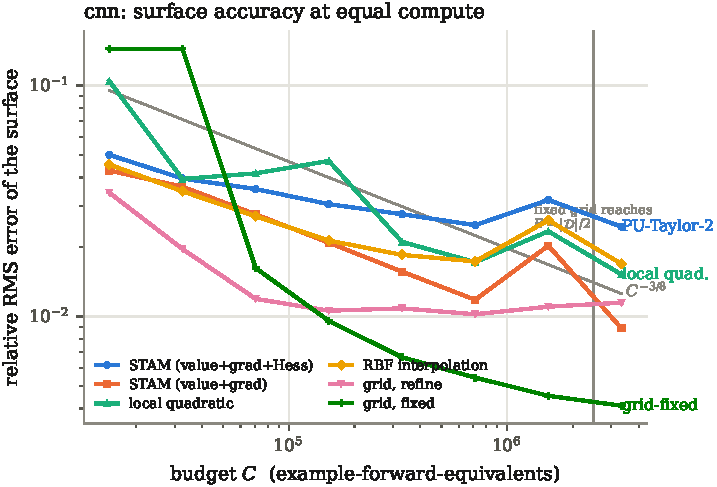
\includegraphics[width=0.72\linewidth]{../figures/budget_error_cnn.pdf}
\caption{Relative RMS error of the rendered surface against compute budget (CNN/CIFAR-10, median of three seeds, log--log). The two grid baselines flatten: they interpolate their own noise, so past a point extra budget buys nothing (\Cref{prop:floor}). The guide line is the predicted $C^{-3/8}$.}
\label{fig:budget}
\end{figure}


\begin{figure}[t]
\centering
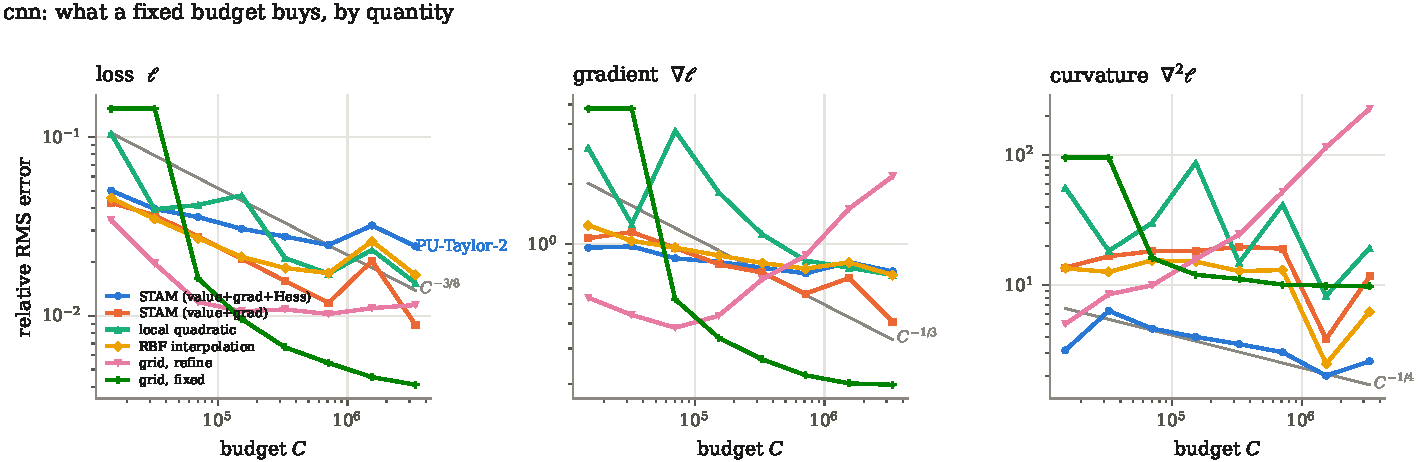
\includegraphics[width=\linewidth]{../figures/rate_separation_cnn.pdf}
\caption{The same sweep scored on three quantities. Derivative probing does not improve the rate for the surface, only its constant --- but it strictly improves the rate for the gradient field and for curvature, which is what \Cref{tab:rates} predicts and what practitioners read off these figures.}
\label{fig:rates}
\end{figure}


\begin{figure}[t]
\centering
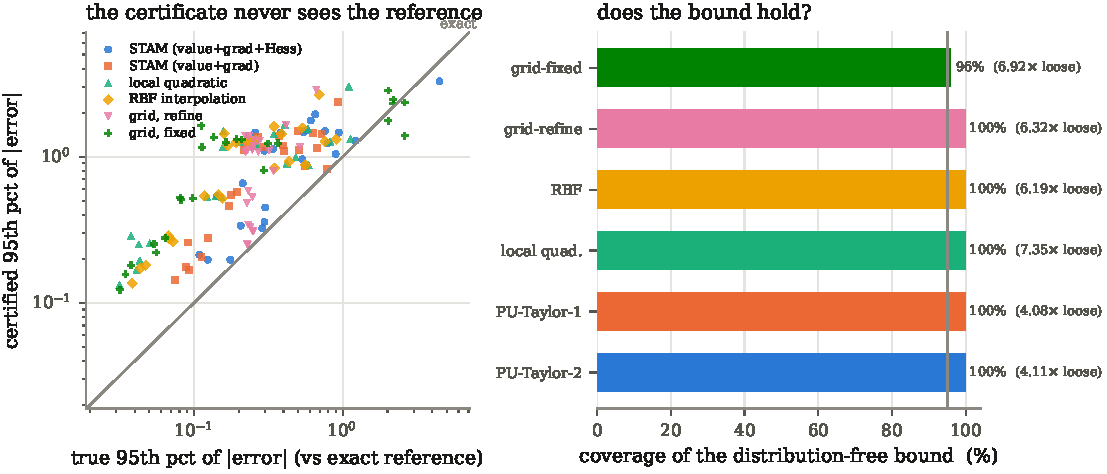
\includegraphics[width=\linewidth]{../figures/certificate_cnn.pdf}
\caption{Left: the certified error against the true error measured against the exact reference. The certificate never sees the reference. Right: empirical coverage of the $95\%$ upper bound, and how tight it is.}
\label{fig:cert}
\end{figure}


\begin{figure}[t]
\centering
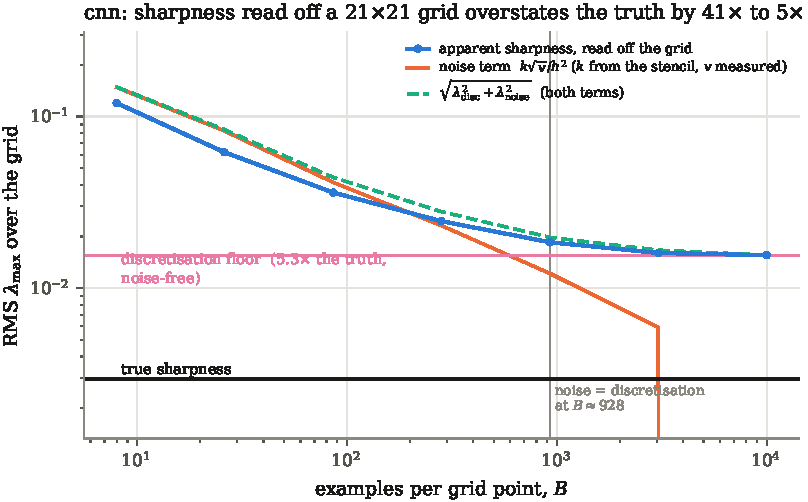
\includegraphics[width=0.68\linewidth]{../figures/sharpness_cnn.pdf}
\caption{Sharpness read off a fixed grid, against the per-point sample size. The apparent value never falls below the noise floor $\lambda_{\mathrm{noise}}\propto\sigma/(h^2\sqrt B)$, whose constant comes from the second-difference stencil and is not fitted. At sample sizes typical of a landscape figure the floor exceeds the signal.}
\label{fig:sharp}
\end{figure}


\begin{figure}[t]
\centering
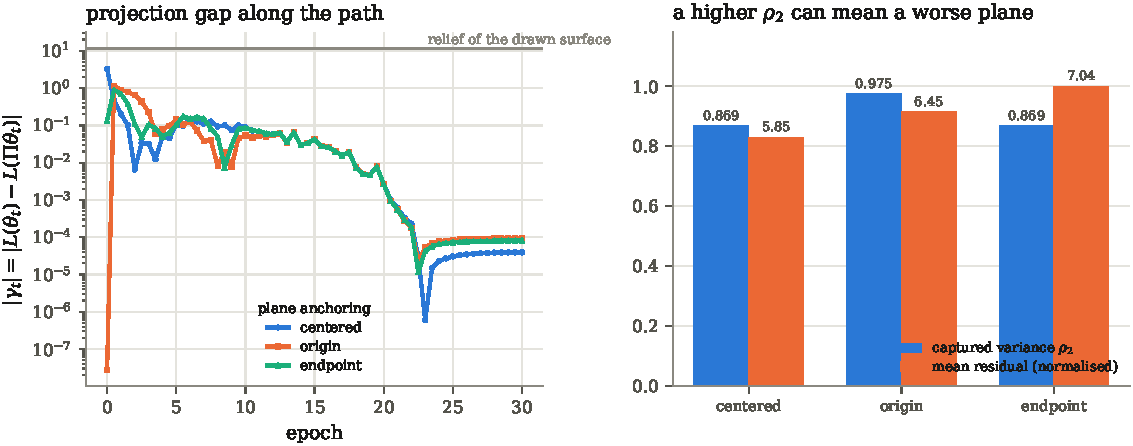
\includegraphics[width=\linewidth]{../figures/fidelity_cnn.pdf}
\caption{Left: the projection gap along the optimiser's path, for three plane constructions. Right: the $\theta_0$-anchored plane reports the highest $\rho_2$ and has the largest residual.}
\label{fig:fid}
\end{figure}


\begin{figure}[t]
\centering
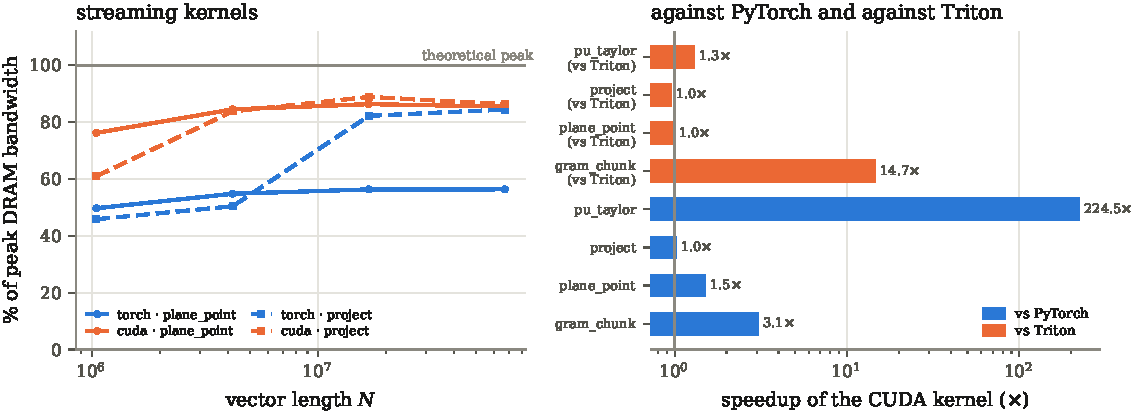
\includegraphics[width=\linewidth]{../figures/kernels.pdf}
\caption{Left: achieved fraction of peak DRAM bandwidth for the two streaming kernels. Right: speedup of the hand-written CUDA kernels over PyTorch and over the Triton implementations.}
\label{fig:kernels}
\end{figure}


\begin{figure}[t]
\centering
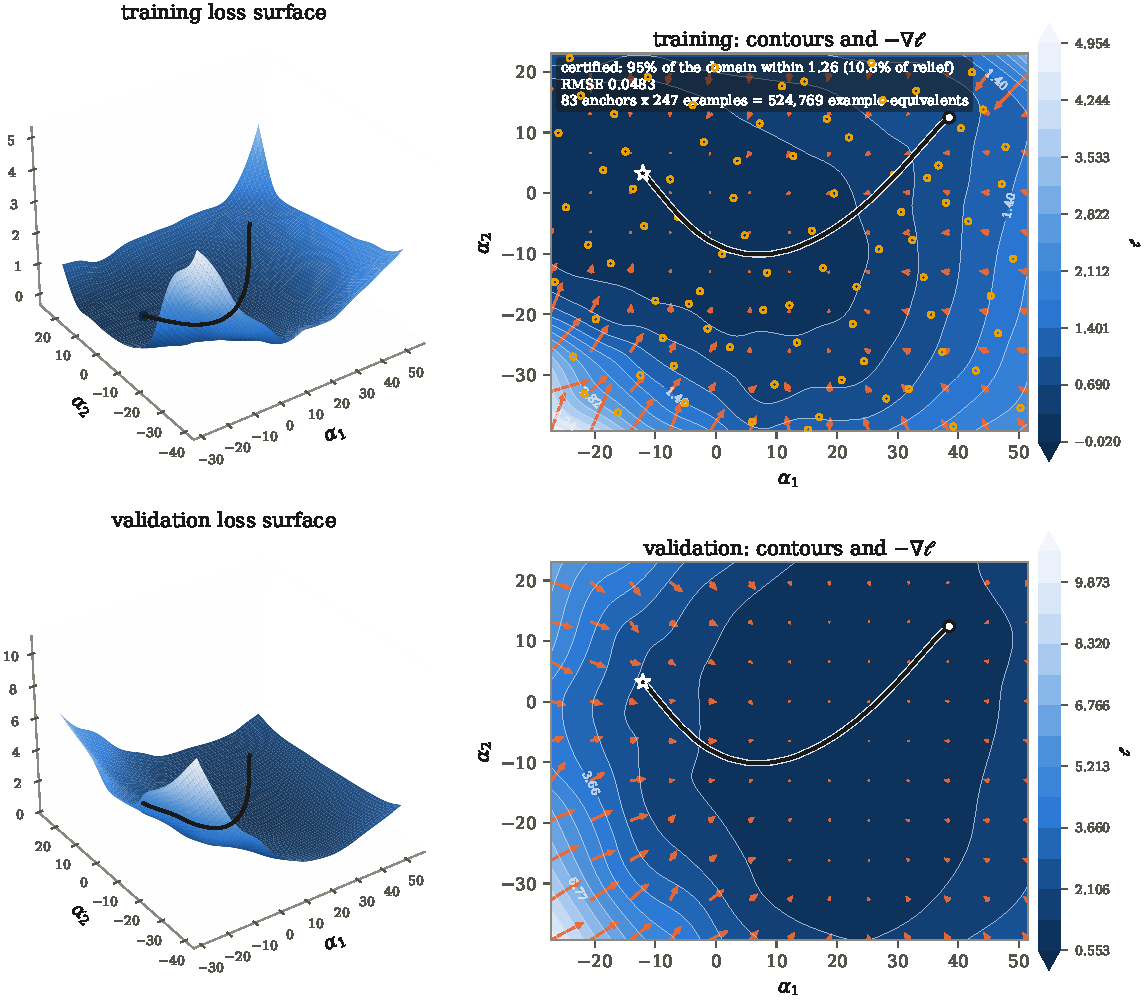
\includegraphics[width=\linewidth]{../figures/landscape_cnn.pdf}
\caption{A certified landscape (CNN/CIFAR-10). Contour intervals are set to at least twice the certified RMS error, so no contour is drawn that the measurement cannot resolve. The quiver field is the exact gradient of the surface, computed analytically from \eqref{eq:pugrad}. Open circles mark the anchors actually probed.}
\label{fig:landcnn}
\end{figure}


\begin{figure}[t]
\centering
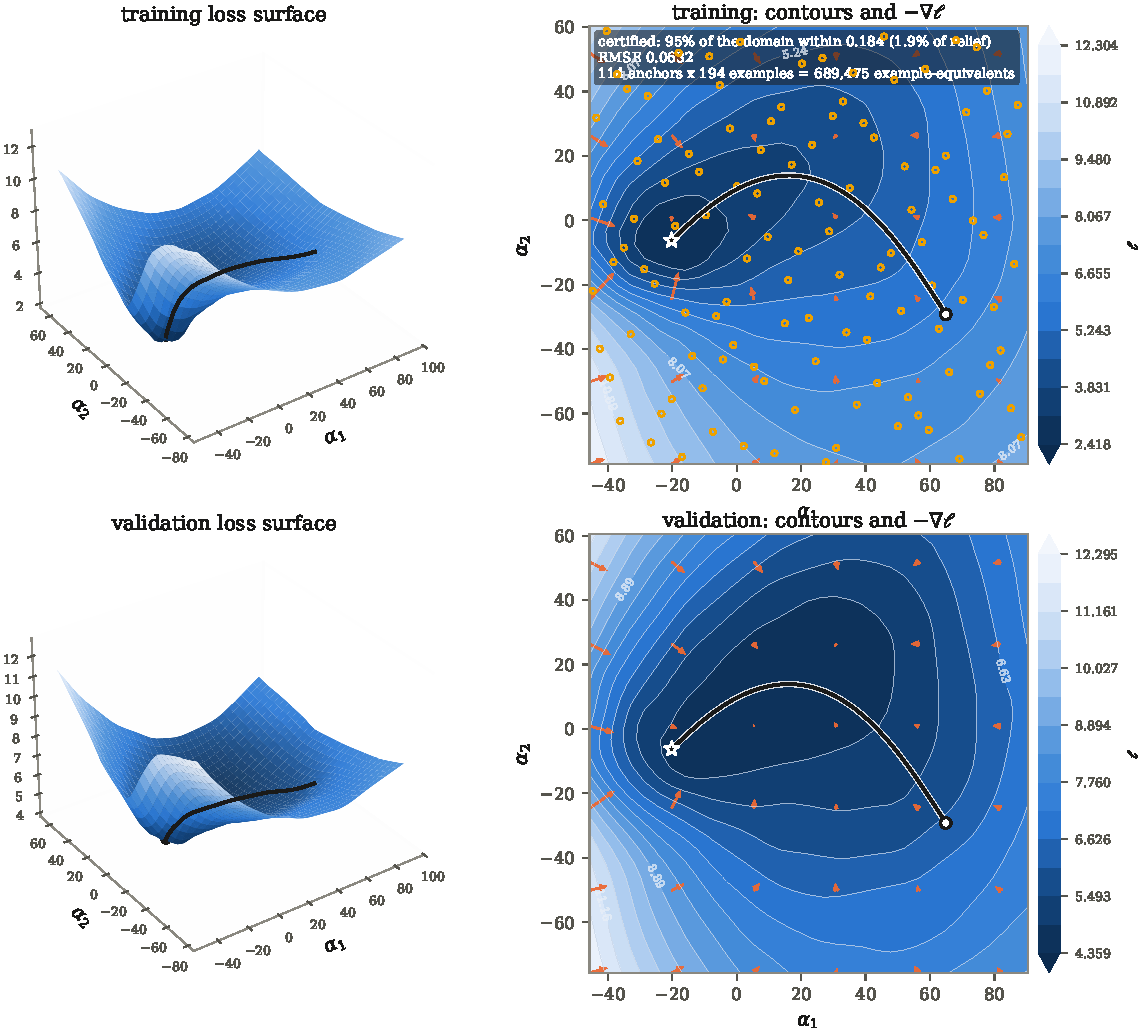
\includegraphics[width=\linewidth]{../figures/landscape_gpt.pdf}
\caption{A certified landscape for the \GPTparams-parameter transformer on WikiText-2.}
\label{fig:landgpt}
\end{figure}


\begin{figure}[t]
\centering
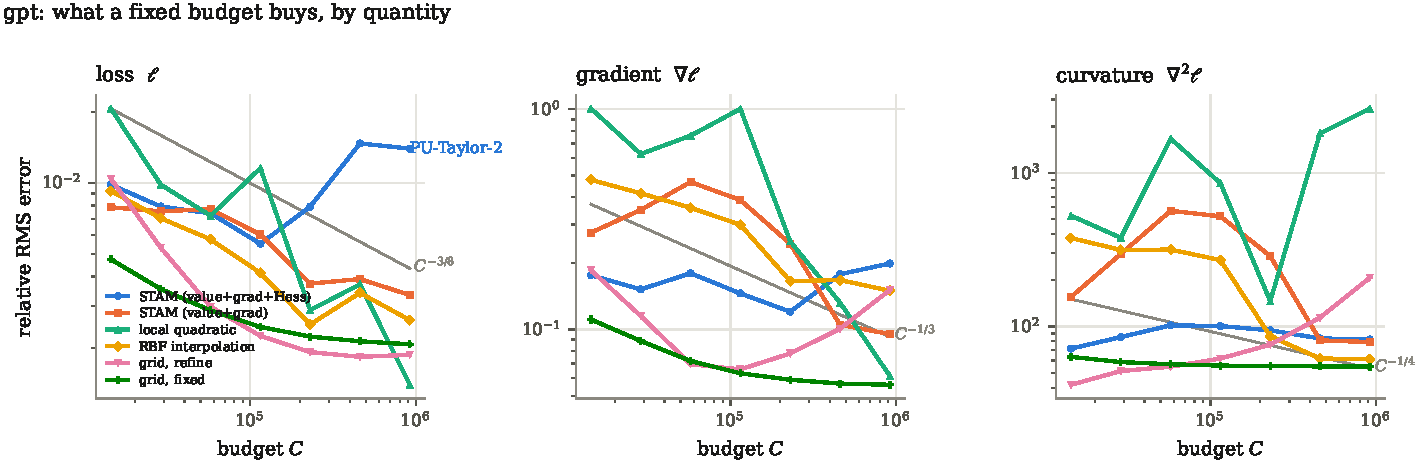
\includegraphics[width=\linewidth]{../figures/rate_separation_gpt.pdf}
\caption{The same sweep on the \GPTparams-parameter transformer. The grid-refinement baseline again degrades with budget on curvature. The relative curvature metric discriminates poorly here because the true curvature is small over a domain where the loss saturates near $\ln|V|$ --- a limitation of the subject, stated in \Cref{sec:limits}.}
\label{fig:ratesgpt}
\end{figure}


\begin{figure}[t]
\centering
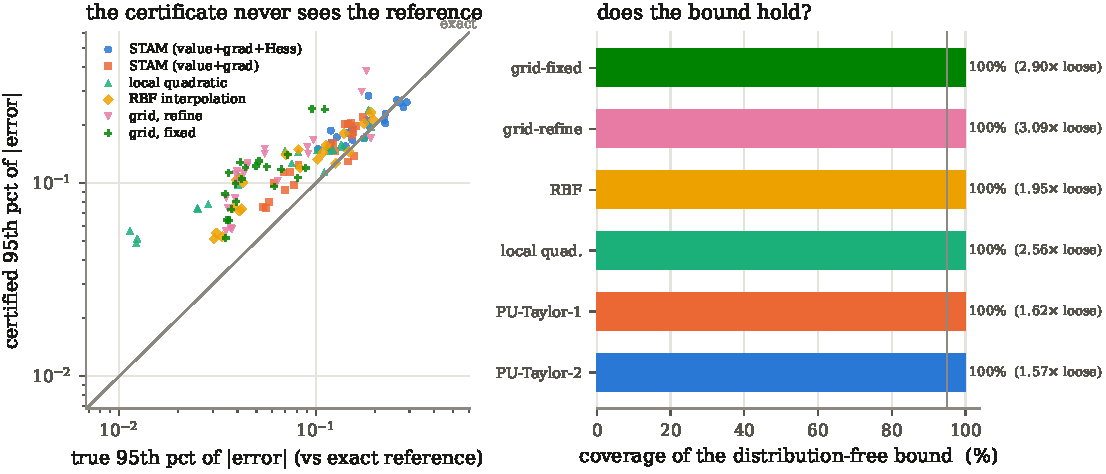
\includegraphics[width=\linewidth]{../figures/certificate_gpt.pdf}
\caption{Certificate validity on the transformer. The error field is far less heavy-tailed than the CNN's, and the certified point estimate is correspondingly close to the truth.}
\label{fig:certgpt}
\end{figure}


\begin{figure}[t]
\centering
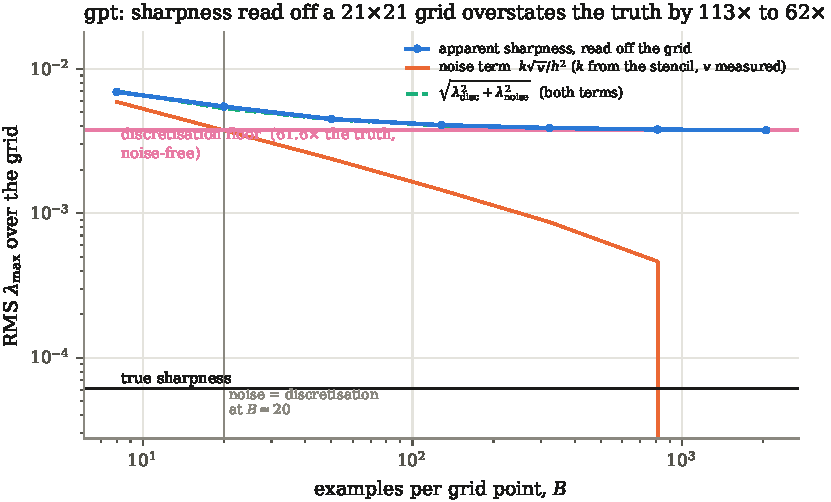
\includegraphics[width=0.68\linewidth]{../figures/sharpness_gpt.pdf}
\caption{Sharpness read off a grid for the transformer: overstated by \GPTsharpworst$\times$ at small samples and still \GPTsharpfloor$\times$ when the probe is exact.}
\label{fig:sharpgpt}
\end{figure}


\begin{figure}[t]
\centering
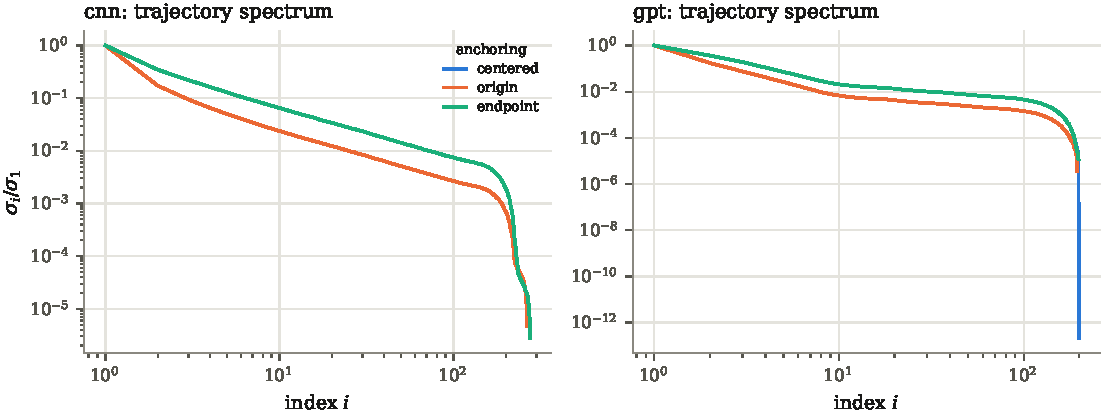
\includegraphics[width=\linewidth]{../figures/spectrum.pdf}
\caption{Trajectory spectra. The uncentred construction concentrates more of \emph{its} ratio in the leading pair, which is why $\rho_2$ favours it while the residual does not.}
\label{fig:spectrum}
\end{figure}


\begin{figure}[t]
\centering
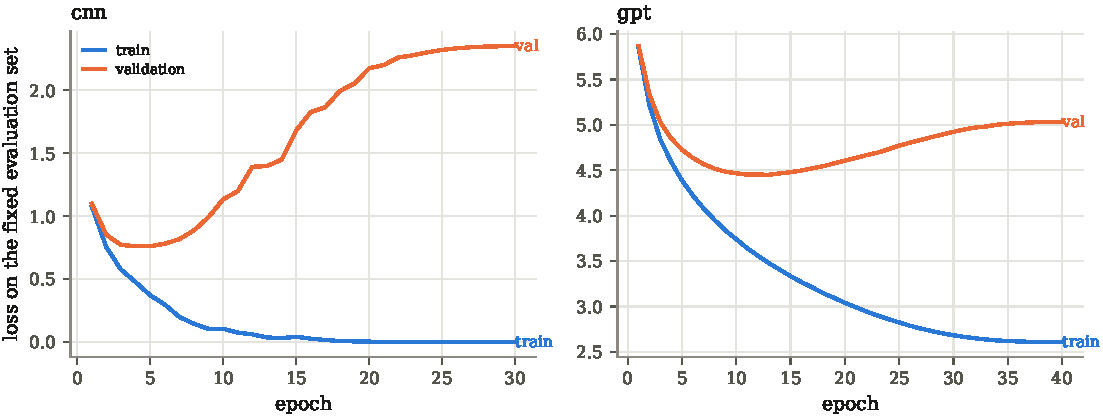
\includegraphics[width=\linewidth]{../figures/training.pdf}
\caption{Training curves on the fixed evaluation sets that define the landscapes.}
\label{fig:training}
\end{figure}


\section{Machine-checked foundations}
\label{sec:lean}

Six statements are formalised in Lean~4 \citep{moura2021lean4} with mathlib
\citep{mathlib2020}:

\begin{center}
\small
\begin{tabular}{ll}
\toprule
Lean name & statement \\
\midrule
\lean{alloc\_lower\_bound}, \lean{alloc\_attained} & \Cref{thm:alloc} \\
\lean{pu\_error\_bound} & \Cref{lem:pu} \\
\lean{interpolation\_floor} & \Cref{prop:floor} \\
\lean{debias\_unbiased} & \Cref{prop:cert} \\
\lean{sum\_dist\_sq\_center} & \Cref{prop:affine} \\
\lean{taylor2\_patch\_bound} & the $\tfrac16M_3h^3$ patch bound \\
\bottomrule
\end{tabular}
\end{center}

\noindent All check with \texttt{\#print axioms} reporting only \texttt{propext},
\texttt{Classical.choice} and \texttt{Quot.sound}; there are no \texttt{sorry}s and no
added axioms.

What is \emph{not} formalised: the minimax lower bound (a citation), the rate
separation of \Cref{tab:rates} (a citation plus a smoothness bookkeeping argument), and
the certificate's concentration bound (a citation). We formalise the parts that are
original arithmetic, which is where an error would be ours.

\section{Limitations}
\label{sec:limits}

\begin{itemize}[leftmargin=1.4em,itemsep=1pt]
\item \textbf{The evaluation sets are small enough that large budgets saturate them.}
With $|\D|=10^4$ (CNN) and $2048$ sequences (transformer), the top of the swept range
lets even the cheapest method draw a large fraction of $\D$ per point, at which stage
the probe is nearly exhaustive and the sampling noise the analysis is about has
essentially vanished. That regime flatters the fixed grid and is not one a real dataset
reaches; it is marked on \Cref{fig:budget}. The transformer is affected more, and its
curvature comparison is further weakened by the true curvature being small over a domain
where the loss saturates near $\ln|V|$, so a \emph{relative} curvature error is large for
every method and discriminates poorly. The CNN is where the budget-limited regime is
properly explored.
\item \textbf{The plane still hides most of the space.} Nothing here makes a $2$-plane
adequate; it makes the inadequacy \emph{measurable}. A large projection gap is a reason
to distrust the figure, and we report it.
\item \textbf{$M_3$ is not finite for ReLU networks} in the classical sense. The
asymptotic rate is therefore a statement about the smoothed, data-averaged loss; the
empirical certificate is what carries the ReLU case, and it assumes nothing.
\item \textbf{The certificate bounds a mean and a quantile, not a supremum.} Finitely
many uniform probes do not support a sup-norm claim.
\item \textbf{Normalisation layers are out of scope.} Scale invariance makes distances
in the plane meaningless; a filter-normalised parameterisation \citep{li2018visualizing}
would need to be composed with this analysis, and the interaction is not studied here.
\item \textbf{Two subjects, one optimiser.} The exponents are measured on a
\CNNparams-parameter CNN and a \GPTparams-parameter transformer under AdamW. The
theory is not model-specific but the constants are.
\end{itemize}

\section{Related work}
\label{sec:related}

\citet{goodfellow2015qualitatively} introduced $1$-D interpolation between parameter
vectors; \citet{li2018visualizing} established the $2$-D random-direction protocol and
filter normalisation, and is the direct ancestor of this work. Trajectory PCA appears in
\citet{li2018visualizing} and \citet{fort2019emergent}. Mode connectivity
\citep{garipov2018loss,draxler2018essentially} and weight averaging
\citep{izmailov2018averaging} rely on such pictures for their qualitative claims. The
low effective dimension of gradient dynamics \citep{gurari2018gradient,sagun2018empirical}
is what makes a $2$-plane informative at all. \emph{None of these report an error on the
rendered surface}, and to our knowledge the accuracy of a landscape figure has not
previously been quantified.

Sharpness is estimated by Hessian eigenvalue methods
\citep{ghorbani2019investigation,yao2020pyhessian} that probe curvature directly at a
point --- and are, in our terms, the $\kappa_2$ path --- while landscape figures
estimate it visually from values. \Cref{tab:rates} quantifies the gap between the two,
which matters because conclusions about flat minima
\citep{keskar2017large,dinh2017sharp,foret2021sharpness} are drawn from both.

The reconstruction is a partition-of-unity method \citep{babuska1997partition} with
Wendland weights \citep{wendland1995piecewise}; the statistical content is classical
nonparametric regression \citep{stone1980optimal,fan1996local,tsybakov2009introduction}.
The contribution is not any of these pieces but the identification of the visualisation
problem with the budgeted-estimation setting, and the consequences that follow.

\section{Discussion}
\label{sec:discussion}

The result we would most like to see acted on is the simplest: \emph{a landscape figure
should state its error}, and doing so costs about $6\%$ of the budget. The rest follows
from taking that requirement seriously --- once the error is measured, the allocation
that minimises it is a well-posed problem with a closed-form answer, and the answer says
to probe fewer places more deeply and to ask for derivatives while you are there.

Three directions are now reachable. Curvature-adaptive anchor placement should improve
the constant, since the pilot already measures where $M_3$ is large. The same analysis
with $k>2$ subspace dimensions trades $O(k)$ Hessian-vector products against an
$O(h^{-k})$ reconstruction cost, and the crossover is computable from the same cost
model. And because the certificate is a stopping rule, a landscape can be refined
adaptively to a requested accuracy rather than to a fixed grid --- which is what one
actually wants.

\FloatBarrier

\bibliographystyle{plainnat}
\bibliography{refs}

\appendix
\section{Reproduction}
\label{app:repro}

\begin{itemize}[leftmargin=1.4em,itemsep=1pt]
\item Hardware: 2$\times$ Quadro RTX 6000 (sm\_75, 23.5\,GiB, 72 SMs), 36 CPU cores.
\item Software: PyTorch 2.7.1+cu118 (CUDA 11.8), Python 3.11.14, cuDNN 90100.
\item Numerical policy selected at run time: reduction accumulator \texttt{float32} (fp64 is rate-limited on this part, so compensated fp32 is used), trajectory storage \texttt{float16}, TF32 unavailable, bf16 tensor cores unavailable.
\item Every result file records the full environment and the fingerprint of the evaluation set it used.
\item Reproduce with \texttt{make all}; the Lean proofs with \texttt{cd proofs/StamCert \&\& lake build}.
\end{itemize}

\end{document}
